\documentclass{article}
\usepackage{graphicx}
\usepackage[margin=1.5cm]{geometry}
\usepackage{amsmath}

\begin{document}

\title{Warm Up: Kinematics in 2D and 3D}
\author{Prof. Jordan C. Hanson}

\maketitle

\section{Memory}

\begin{enumerate}
\item $y(t) = -\frac{1}{2}g t^2 + v_{i,y} t + y_i$ ... Accelerating system vertically.
\item $x(t) = v_{i,x} t + x_i$ ... Constant velocity horizontally.
\item $v_f^2 = v_i^2 + 2 a (x_f - x_i)$ ... Kinematic equation without time.
\end{enumerate}

\section{Kinematics in 2D and 3D}

\begin{enumerate}
\item Imagine a system propagating through 3D space with a velocity vector $\vec{v} = (2t^2-t)\hat{i} + 2t\hat{j}$.  (a) Write the acceleration vector by taking the derivative. (b) What is $\vec{a}(0.5)$? \\ \vspace{1cm}
\item Suppose a system is thrown into the air, accelerating downwards due to gravity, but proceeding horizontally at constant velocity.
\begin{itemize}
\item We have shown in a previous calculation that the trajectory follows $y(x) = -a x^2 + b$, with $b = \tan\theta$ and $a = \frac{1}{2} g/v_{i,x}^2$.
\item Note in Fig. \ref{fig:1} that breaks the initial velocity $v_i$ into two components:
\begin{figure}[ht]
\centering
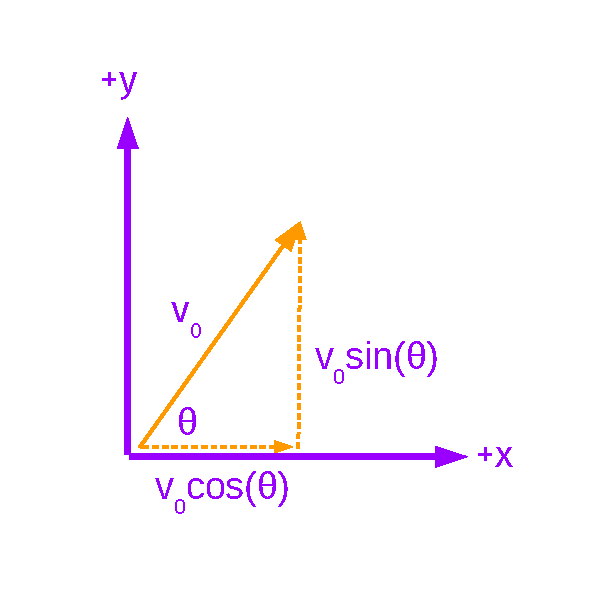
\includegraphics[width=0.25\textwidth]{figures/Vectors1.pdf}
\caption{\label{fig:1}}
\end{figure}
\item Convince yourself that the x-component of the initial velocity is $v_{i,x} = v_i \cos\theta$, and $v_{i,y} = v_i \sin\theta$ by performing Pythagorean theorem to get the hypoteneuse. \\ \vspace{0.5cm}
\item Suppose a system is launched at a 60 degree angle with speed $v_i = 20$ m/s from the origin.  (a) Where will it land? (b) How fast is it going when it lands?
\end{itemize}
\end{enumerate}

\end{document}
